%------------- PROG1P3 - REPORT -------------%
%--------------------------------------------%
%- @authors Simon Bihel - Florestan De Moor -%
%- @version 1.0 -----------------------------%
%--------------------------------------------%

\documentclass[a4paper]{article}

\usepackage[english]{babel}
\usepackage[utf8]{inputenc}
\usepackage[T1]{fontenc} 
\usepackage[margin=2.5cm]{geometry}
\usepackage{graphicx}
\usepackage{xspace}

\usepackage{amsmath}
\usepackage{amsfonts}
\usepackage{amssymb}

%% Tikz for picture drawing %%
\usepackage{tikz}
\usetikzlibrary{arrows}

\usepackage{xcolor,colortbl}

\usepackage{caption}
\usepackage{subcaption}
\usepackage{float}

\setlength{\parskip}{6mm plus2mm minus2mm}


%% Specific commands %%
\newcommand{\this}{\emph{Ant vs. SomeBees }}


%% Path of the pictures %%
\graphicspath{{../src/main/resources/img/}{screens/}}

\begin{document}

\title{PROG1 P3 - Ant vs. SomeBees}
\author{Simon Bihel, Florestan De Moor \\ ENS Rennes, Computer Science Department, 1st year}
\date{December 13rd, 2015}


\maketitle

\section*{Introduction}
% TODO Florestan / Simon

	In this report, we present our work on the third project of the programming course. It consisted in creating a game based on the famous one \emph{Plants vs. Zombies$^\copyright$}. \this was programmed using the Scala language, and the Scala-swing library for the graphic interface. This project was done using mostly the OOP paradigm, but also some FP.
	
	First, we will introduce the game and its features. Then, we will expose the class diagram, and the structure we decided to use to create this game. Finally, we will clarify some parts of the implementation.


\section{Game overview}

\this is a tower defense like game. The terms are really simple : the player controls an anthill, which has five tunnels. An army of bees will try to invade it. The goal is to survive as long as possible by killing the bees entering the tunnels in waves. If a bee succeed to go through a whole tunnel, the game is lost. Each bee killed gives the player 5 points, the player score is printed in the bottom information bar.

\begin{figure}[H]
	\center
	\foreach \x in {1,...,6} {
\includegraphics[scale=0.3]{tunnel.png}}
\includegraphics[scale=0.3]{tunnel_water.png}
	\caption{Example of tunnel}
	\label{tunnel}
\end{figure}

\paragraph{Defending the tunnels} In order to defend the tunnels, the player has the possibility to put some ants. This has a cost : food. The starting food amount is 2. The food amount is printed in the bottom bar. Each ant has specific cost, armour, and abilities. For example, the harvester ant collect 1 food per turn, while thrower ants can throw projectiles to attack bees. The bodyguard is a special unit, that can be put at the same place than another ant, in order to protect it.

\begin{figure}[H]
	\center
	
\includegraphics[scale=0.5]{ant_harvester.png}
	
\includegraphics[scale=0.5]{ant_fire.png}
	
\includegraphics[scale=0.5]{ant_longthrower.png}
	
\includegraphics[scale=0.5]{ant_scuba.png}
	\caption{Some ants}
	\label{someants}
\end{figure}

\paragraph{Turns} The game is divided in turns. The bees are continuously moving at each frame, but actions such as food collecting or shooting are performed at each turn.

\paragraph{Bee waves} The first bee will come in after six turns, and one bee will appear at each turn from then on. The wave difficulty will increase : incoming bees will have greater armour, and damages up. There are two types of bees : the black ones, that can attack ants when they are right in front of them, and the red ones, that can shoot afar. A new bee appears in one of the five tunnels, picked up randomly.

\begin{figure}[H]
	\center
	
\includegraphics[scale=0.5]{bee.png}
	
\includegraphics[scale=0.5]{rangebee.png}
	\caption{Bees}
	\label{bees}
\end{figure}

\paragraph{Spells} The player has also the possibility to use spells. This also costs food. Three spells were implemented :
 
\begin{center}
	\begin{tabular}{|c|p{13cm}|}
		\hline
		\rule[1mm]{0pt}{5mm}
		\raisebox{-.5\height}{
\includegraphics[scale=0.5]{freeze.png}}
		   & The freeze ability can be applied on a place of the tunnel, and has for consequence to freeze all bees within for three turns. Notice that they are unable to move, but not to shoot. \\
		\hline
		\rule[1mm]{0pt}{5mm}
		\raisebox{-.5\height}{
\includegraphics[scale=0.5]{radar.png}}
		 & The radar ability can be given to an ant. As long as the concerned ant is living, the player will be able to see the armour points of all bees in the specific tunnel. \\
		\hline
		\rule[1mm]{0pt}{5mm}
		\raisebox{-.5\height}{
\includegraphics[scale=0.5]{double.png}}
		 & The upgrade spell is very powerful : it can be applied to an ant, in order to level it up. This doubles its damage power. Notice that it doesn't modify armour points, the player has to protect well its upgraded ants. \\
		\hline
	\end{tabular}
\end{center}

\paragraph{GUI} The user interface contains a menu which allows the player to select a type of ant, or a spell. There is also a remove button, to delete existing ants. Notice that deleting an ant doesn't give back food. A message can be displayed in the bottom bar.

\begin{figure}[H]
	\center
	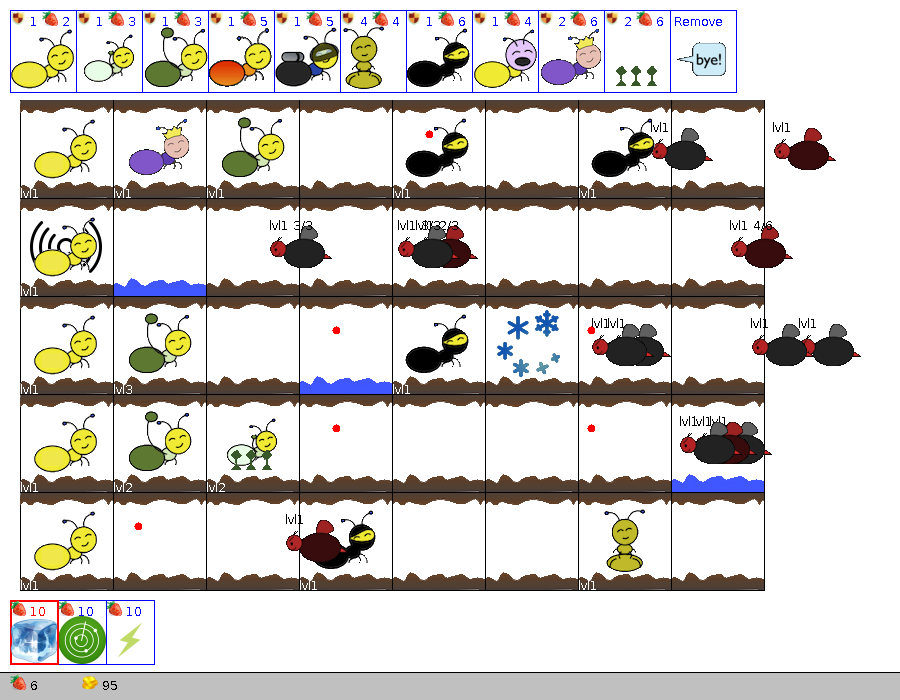
\includegraphics[scale=0.3]{screen2.png}
	\caption{Graphic User Interface}
	\label{gui}
\end{figure}


\section{Program's structure}
% TODO Simon

The architecture of the program is based on a Model-View-Controller pattern. The View part displays the UI and warns the Controller of inputs. The Controller then decides what action should be done in response and asks the Model to do it. The latter, which only stores the elements of the game, executes the request.
The game itself is composed of Places that contains Ants and Bees that fire Projectiles at each others.
The overall interactions of the various parts of the program are shown in figure~\ref{classDiagram}.

\begin{figure}[H]
	\centering
	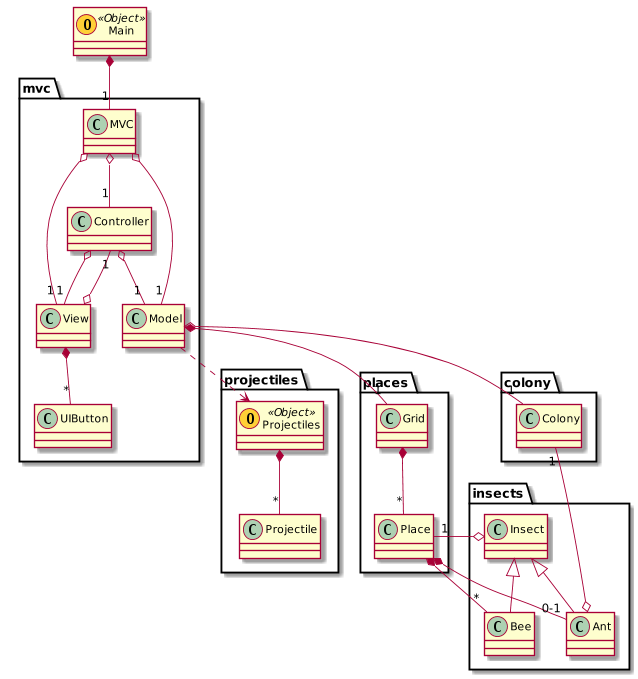
\includegraphics[scale=0.7]{classDiagram.png}
	\caption{Global class diagram}
	\label{classDiagram}
\end{figure}
%% LEGEND OF THE DIAGRAM ? %%

	\subsection{Graphic User Interface}
	As we have previously said, the GUI, and thus the View part of the MVC, has two roles : displaying and warning the Controller of inputs. For the first part, it takes the elements of the game as parameters and draw them, along with the Buttons. Secondly, only clicks are used, so there is just to check that the click is on a valid area (i.e. on a Button or on a Place) and then tell the Controller that something has been clicked.
	
	\subsection{Game engine}
	As it is turn-based, the game is run by two running timers : one for the frames and a second one for the moves of the insects. On each frame (~60 per second) movements are executed, bees move to the right and projectiles get closer to their target. On each move (~1 per second) the insects execute their actions like attacking.


\section{Implementation clarifications}
% TODO Florestan

\paragraph{Bee waves} bla bla turns with levels, one turn a normal bee, the other a beerange, counter to start after 6 turns, life increasing with number of the wave

\paragraph{Button menu} bla bla selecting a button, method isclicked, then if is clicked perform an action by the method action, which send to model (or controller, have to check) and then try to add for instance, exception ClickFound to stop searching when useless

\paragraph{Spells} additional features for spells : booleans to know for the drawing of the place, overlay for drawing, counter for the freeze spell, to unfreeze after 3 turns, radar, upgrade tower to level up

\paragraph{Information bar} Sometimes, the player is trying to make illegal actions, so it is necessary to display a warning. To do this, we created an object \emph{Msg} in View part.

\begin{tabular}{c p{12cm}}
	\raisebox{-.5\height}{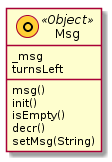
\includegraphics[scale=0.6]{msgDiagram.png}}
	& When a message needs to be displayed, for example when an exception \emph{NotEnoughFood} or \emph{NotEmptyPlace} is caught, we have a method to set a message. It modifies the number of turns left during which the message will be displayed. In the Model part, if the message isn't empty, this number is decreased by one at each turn, and the message is re-initialized when zero is reached.\\
\end{tabular}

\paragraph{Timers} 2 timers, one to manage the frames, and the other the turns

%% TELLME What else ? %%



\section{Possible improvements}
% TODO Florestan / Simon
bla bla la lorem ipsum

% bla bla here before

\paragraph{AI} A possible extension would be to simulate an artificial intelligence, to manage the waves of bees. It would know the state of the game, and would choose at each wave the best tunnel to try to exploit the player weaknesses.

\paragraph{Events}


\section*{Conclusion}
% TODO Florestan / Simon
bla bla la lorem ipsum


\end{document}